\documentclass[../../Aurora C# unofficial manual.tex]{subfiles}

\begin{document}
	\section{Deleting asteroids and Lagrange points}\label{7_deleting asteroids_and_lagrange}
	Original post can be found
	\href{http://aurora2.pentarch.org/index.php?topic=8495.msg118803#msg118803}{here}.
	\\\\
	
	Deleting individual asteroids can be done by using the Delete Body button. To delete an entire asteroid belt or all the Trojan asteroids for a particular planet, click one of the asteroids in the belt or one of the Trojans and click Delete Asteroids. There will be two warnings before all the affected asteroids are deleted.
	
	Lagrange Points can be removed by selecting the parent system body and clicking Remove Lagrange.
	
	Below is the final version of the System View in SM mode with all system engineering buttons present.
	\begin{figure}[H]
		\centering
		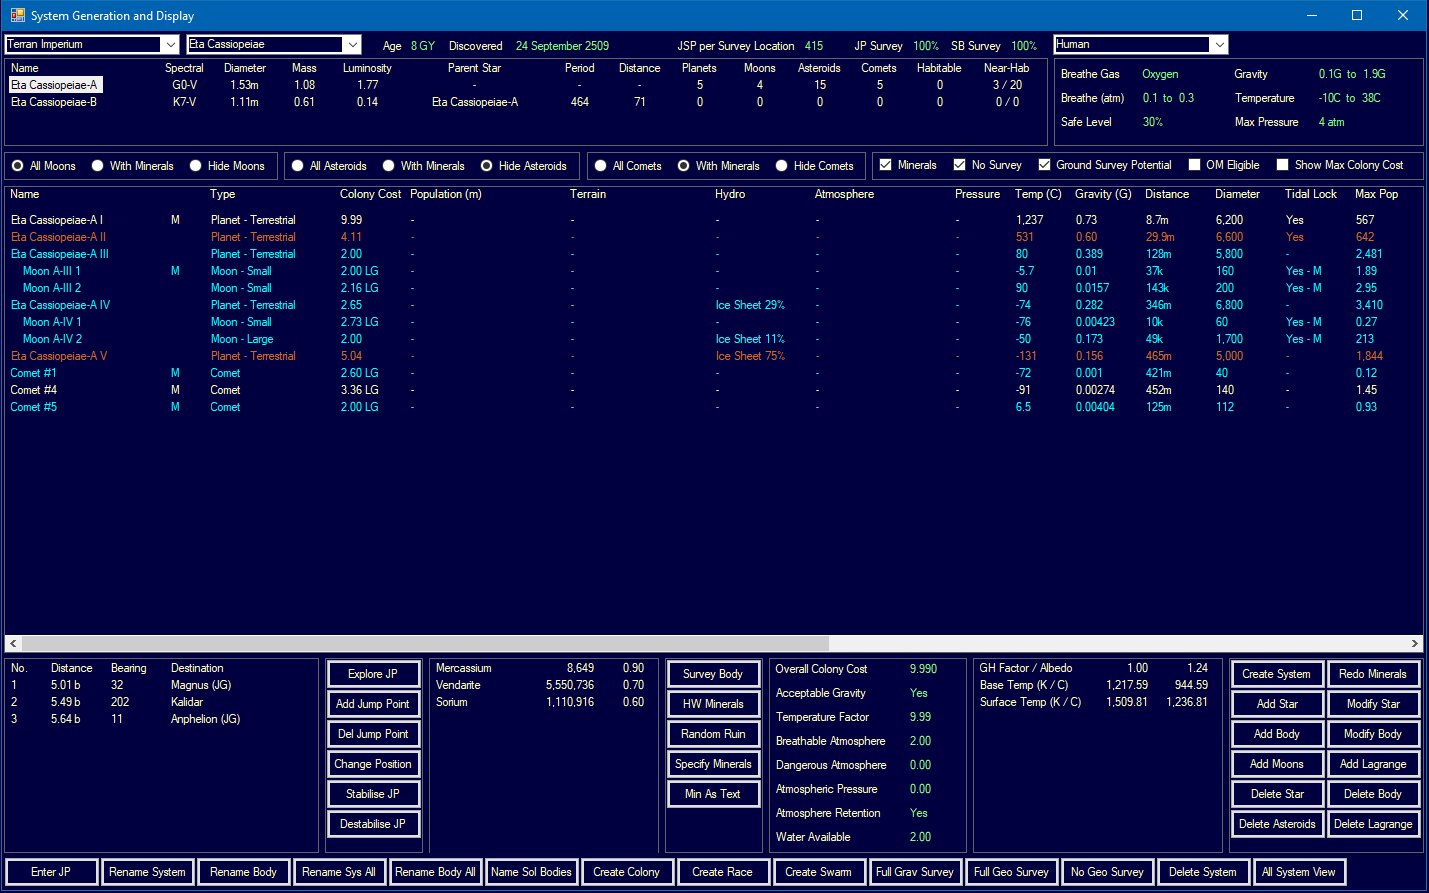
\includegraphics[width=0.95\linewidth]{images/DeletingLagrangePoints}
		\caption[Deleting Lagrange Points]{Deleting Lagrange Points}
		\label{fig:deletinglagrangepoints}
	\end{figure}	
\end{document}